\documentclass{beamer}
\usetheme{Madrid}
% \usetheme{Frankfurt}
% \usetheme{Darmstadt}
% \usetheme{Berlin}
% \usetheme{Warsaw}
% \usetheme{Berkeley}
% \usetheme{Bergen}
% \usetheme{CambridgeUS}
% \usetheme{Copenhagen}

\providecommand{\pr}[1]{\ensuremath{\Pr\left(#1\right)}}
\providecommand{\cbrak}[1]{\ensuremath{\left\{#1\right\}}}
\providecommand{\brak}[1]{\ensuremath{\left(#1\right)}}
\newcommand{\mysolution}{\noindent \textbf{Solution: }}
\newcommand{\myvec}[1]{\ensuremath{\begin{pmatrix}#1\end{pmatrix}}}

\title{AI1110 - Probability and Random Variables \\
        Assignment 7}
\author{Abhinav Yadav \\ 
        cs21btech11002}

\begin{document}
    \maketitle
    % \begin{frame}{Table of Contents}
    %     \tableofcontents
    % \end{frame}

    \begin{frame}{CBSE class 12 Exercise 13.4}
        \begin{section}{Question}
            \begin{block}{Question 6}
                From a lot of 30 bulbs which include 6 defectives, a sample of 4 bulbs is drawn
                at random with replacement. Find the probability distribution of the number of
                defective bulbs.
            \end{block}
        \end{section}
    \end{frame}

    \begin{frame}{Solution}
        \section{Solution}
        Let us define \textbf{success} as \textbf{Ball drawn is not defective}\\
        Then probability of success is $p=\frac{6}{30}=\frac{4}{5}$\\
        and probability of failure is $q=\frac{1}{5}$\\

        Let the random variable $X\in\cbrak{0, 1, 2, 3, 4}$ denote the number of defective bulbs\\
        This is Bernauli trial. The probability of $i\in\cbrak{0, 1, 2, 3, 4}$ balls being defective is given by
        \begin{align}
            \pr{X=i} = \myvec{4\\i}p^iq^{4-i}
        \end{align}
        Therefore, the probability distribution is
    \end{frame}
    \begin{frame}
        \begin{table}
            \begin{tabular}{|c|c|}
                \hline
                \textbf{No. of defective balls} & \textbf{Probability}\\
                \hline
                0 & \myvec{4\\0}$\times$\brak{\frac{4}{5}}$^4$ = $\frac{256}{625}$\\
                \hline
                1 & \myvec{4\\1}$\times\frac{1}{5}\times$\brak{\frac{4}{5}}$^3$ = $\frac{256}{625}$\\
                \hline
                2 & \myvec{4\\2}$\times\brak{\frac{1}{5}}^2\times$\brak{\frac{4}{5}}$^2$ = $\frac{96}{625}$\\
                \hline
                3 & \myvec{4\\3}$\times\brak{\frac{1}{5}}^3\times$\brak{\frac{4}{5}}$^1$ = $\frac{16}{625}$\\
                \hline
                4 & \myvec{4\\4}$\times\brak{\frac{1}{5}}^4\times$\brak{\frac{4}{5}}$^0$ = $\frac{1}{625}$\\
                \hline
            \end{tabular}
        \end{table}
    \end{frame}

    \begin{frame}{Code}
        \section{Code}
        \begin{figure}
            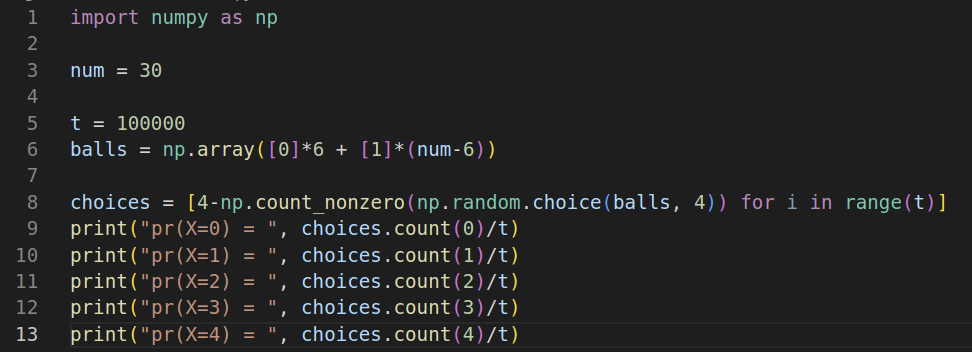
\includegraphics[width=\textwidth]{images/PythonCode.png}
            \caption{1}
            \label{Fig:code}
        \end{figure}
    \end{frame}

\end{document}